%!TeX program = xelatex
\documentclass[12pt,hyperref,a4paper,UTF8]{ctexart}
\usepackage{SJTUReport}
\usepackage{tikz}
\usepackage{geometry}
\usepackage{graphicx}
\usepackage{float}

%%-------------------------------正文开始---------------------------%%
\begin{document}

%%-----------------------封面--------------------%%
\cover

%%------------------摘要-------------%%
\begin{abstract}

本项目设计并实现了一个基于Web的网络端口扫描工具,旨在为网络安全测试提供直观、高效的端口扫描解决方案。系统采用C++后端和HTML5前端相结合的架构,支持多种扫描方式包括TCP SYN扫描、TCP Connect扫描、TCP FIN扫描、UDP扫描以及ICMP ping检测。

系统主要功能包括:多线程高速端口扫描、实时扫描进度显示、扫描结果可视化展示、扫描历史记录管理、以及基于开放端口的网络安全风险评估。后端采用httplib库构建RESTful API服务,前端使用现代Web技术实现响应式用户界面。

通过实际测试验证,系统能够准确识别目标主机的开放端口,扫描速度达到每秒数百个端口,具有良好的稳定性和用户体验。该工具为网络安全专业人员提供了一个功能完善、易于使用的端口扫描解决方案。

\end{abstract}

\thispagestyle{empty} % 首页不显示页码

%%--------------------------目录页------------------------%%
\newpage
\tableofcontents

%%------------------------正文页从这里开始-------------------%
\newpage
\section{需求分析}

\subsection{项目背景}
随着网络技术的快速发展,网络安全问题日益突出。端口扫描作为网络安全评估的基础工具,对于发现网络漏洞、评估系统安全性具有重要意义。传统的命令行端口扫描工具虽然功能强大,但缺乏直观的用户界面,对于非专业用户来说使用门槛较高。

\subsection{项目需求}
本项目旨在开发一个基于Web的网络端口扫描工具,主要解决以下问题:

\begin{enumerate}
    \item \textbf{用户友好性}:提供直观的图形用户界面,降低使用门槛
    \item \textbf{功能完整性}:支持多种扫描方式,满足不同场景需求
    \item \textbf{性能优化}:采用多线程技术提高扫描效率
    \item \textbf{结果可视化}:以图表形式展示扫描结果,便于分析
    \item \textbf{历史管理}:保存扫描历史,支持结果对比和趋势分析
\end{enumerate}

\subsection{功能目标}
系统需要实现以下核心功能:

\begin{itemize}
    \item \textbf{ICMP扫描}:检测目标主机是否可达
    \item \textbf{TCP SYN扫描}:快速识别开放端口,避免建立完整连接
    \item \textbf{TCP Connect扫描}:建立完整TCP连接进行端口检测
    \item \textbf{UDP扫描}:检测UDP端口状态
    \item \textbf{多线程扫描}:支持自定义线程数,提高扫描效率
    \item \textbf{实时进度显示}:显示扫描进度和状态
    \item \textbf{结果可视化}:以表格和图表形式展示扫描结果
    \item \textbf{历史记录}:保存和管理扫描历史
    \item \textbf{结果导出}:支持扫描结果导出功能
\end{itemize}

\section{总体设计}

\subsection{系统架构}
系统采用前后端分离的架构设计,如图\ref{fig:architecture}所示:

\begin{figure}[h]
\centering
\begin{tikzpicture} [
    box/.style={rectangle, draw, rounded corners, minimum width=2cm, minimum height=1cm, align=center},
    arrow/.style={->, thick}
]
    % 前端层
    \node[box, fill=blue!20] (web) at (0,3.5) {Web前端\\HTML5/CSS/JS};
    
    % API层
    \node[box, fill=green!20] (api) at (0,1.5) {RESTful API\\httplib};
    
    % 后端服务层
    \node[box, fill=yellow!20] (backend) at (0,0) {C++后端服务};
    
    % 功能模块层
    \node[box, fill=orange!20] (icmp) at (-3.5,-2) {ICMP模块\\ping.h/cpp};
    \node[box, fill=orange!20] (port) at (0,-2) {端口扫描模块\\PortScanner.h/cpp};
    \node[box, fill=orange!20] (network) at (3.5,-2) {网络模块\\network.h/cpp};

    % 连接(加长箭头)
    \draw[arrow] (web) -- ++(0,-0.9) -| (api);
    \draw[arrow] (api) -- ++(0,-0.9) -| (backend);
    \draw[arrow] (backend) -- ++(-0.5,-0.9) -| (icmp);
    \draw[arrow] (backend) -- ++(0,-0.9) -| (port);
    \draw[arrow] (backend) -- ++(0.5,-0.9) -| (network);
\end{tikzpicture}
\caption{系统总体架构图}
\label{fig:architecture}
\end{figure}

% ===================== 2.2 模块划分 =====================

\subsection{模块划分}

本系统按照功能和职责划分为以下五个主要模块,每个模块各司其职、协同工作,具体如下:

\begin{enumerate}
    \item \textbf{Web前端模块}
    \begin{itemize}
        \item 负责为用户提供友好、直观的操作界面,实现参数输入、扫描控制、结果展示、历史记录管理等功能。
        \item 采用HTML5、CSS3和JavaScript等现代Web技术,支持响应式布局,兼容多种终端设备。
        \item 通过AJAX或Fetch API与后端RESTful API进行数据交互,实现无刷新操作体验。
        \item 主要页面包括:扫描配置页、扫描结果页、历史记录页等。
    \end{itemize}

    \item \textbf{RESTful API模块}
    \begin{itemize}
        \item 作为前后端通信的桥梁,负责接收前端请求、参数校验、任务分发和结果返回。
        \item 基于httplib库实现,支持多种HTTP方法(如GET、POST),以JSON格式进行数据交换。
        \item 提供端口扫描、ICMP检测、历史记录管理等接口,保证接口的安全性和稳定性。
        \item 具备错误处理和异常反馈机制,确保前端能够获得明确的操作结果。
    \end{itemize}

    \item \textbf{ICMP扫描模块}
    \begin{itemize}
        \item 实现对目标主机的ICMP Ping检测,用于判断主机是否在线及网络延迟。
        \item 支持自定义超时时间和重试次数,能够返回详细的RTT(往返时延)和丢包率信息。
        \item 采用原始套接字进行ICMP报文的构造与解析,兼容IPv4协议。
        \item 结果通过API模块返回前端,辅助用户判断目标主机状态。
    \end{itemize}

    \item \textbf{端口扫描模块}
    \begin{itemize}
        \item 实现多种端口扫描方式,包括TCP SYN扫描、TCP Connect扫描、TCP FIN扫描和UDP扫描。
        \item 支持自定义端口范围、扫描类型和线程数,提升扫描效率和灵活性。
        \item 采用多线程技术并发扫描,显著提升大规模端口扫描的速度。
        \item 能够统计开放端口、过滤端口、扫描耗时等信息,便于后续分析。
    \end{itemize}

    \item \textbf{网络工具模块}
    \begin{itemize}
        \item 提供底层网络操作的支持,包括IP地址解析、套接字管理、数据包发送与接收等。
        \item 为ICMP和端口扫描模块提供统一的网络接口,简化上层模块的开发。
        \item 封装常用网络操作,提升代码复用性和可维护性。
    \end{itemize}
\end{enumerate}

各模块之间通过清晰的接口进行通信,既保证了系统的高内聚、低耦合,也便于后续功能扩展和维护。

\section{详细设计}

\subsection{Web前端模块设计}

\subsubsection{模块概述}
Web前端模块负责提供用户界面和交互功能,采用响应式设计,支持桌面和移动设备访问。

\subsubsection{主要数据结构}
\begin{itemize}
    \item \textbf{扫描配置对象}:包含目标地址、端口范围、扫描类型等参数
    \item \textbf{扫描结果对象}:包含开放端口、扫描统计、时间戳等信息
    \item \textbf{历史记录对象}:包含历史扫描的配置和结果
\end{itemize}

% 替换“Web前端模块设计”中的核心函数设计

% ---- Web前端模块设计核心函数设计部分删除,因无C++实现 ----

\subsection{后端API模块设计}

\subsubsection{模块概述}
后端API模块基于httplib库构建,提供RESTful风格的HTTP接口,处理前端请求并调用相应的功能模块。

\subsubsection{主要数据结构}
\begin{itemize}
    \item \textbf{请求参数结构}:包含扫描类型、目标地址、端口范围等
    \item \textbf{响应结果结构}:包含状态码、数据内容、错误信息等
    \item \textbf{扫描任务结构}:包含任务ID、状态、进度等信息
\end{itemize}

\subsubsection{核心函数设计}

% 真实函数声明和说明:
\textbf{函数声明}:
\begin{verbatim}
bool TestPortConnection(std::string ip, int port);
\end{verbatim}
\textbf{说明}:测试指定IP和端口是否开放

\textbf{函数声明}:
\begin{verbatim}
std::vector<int> TCPSynScanJson(const std::string& ip, const std::vector<int>& ports);
\end{verbatim}
\textbf{说明}:对指定IP和端口列表进行TCP SYN扫描,返回开放端口列表

\textbf{函数声明}:
\begin{verbatim}
std::vector<int> TCPFinScanJson(const std::string& ip, const std::vector<int>& ports);
\end{verbatim}
\textbf{说明}:对指定IP和端口列表进行TCP FIN扫描,返回开放端口列表

\textbf{函数声明}:
\begin{verbatim}
std::vector<int> tcpConnectScanJson(const std::string& ip, const std::vector<int>& ports);
\end{verbatim}
\textbf{说明}:对指定IP和端口列表进行TCP Connect扫描,返回开放端口列表

\textbf{函数声明}:
\begin{verbatim}
void UDPScan(const std::string& ip, int option);
\end{verbatim}
\textbf{说明}:对指定IP进行UDP端口扫描

\subsection{ICMP扫描模块设计}

\subsubsection{模块概述}
ICMP扫描模块实现ping功能,用于检测目标主机的可达性,支持自定义超时时间和重试次数。

\subsubsection{主要数据结构}
\begin{itemize}
    \item \textbf{ICMP头部结构}:包含类型、代码、校验和等字段
    \item \textbf{Ping结果结构}:包含可达性状态、RTT时间、丢包率等
    \item \textbf{网络地址结构}:包含IP地址、端口等信息
\end{itemize}

% 由于ICMP相关函数未在PortScanner.h中出现,此处可留空或注明见ICMP模块

% 真实ICMP扫描相关函数声明和说明:
\textbf{函数声明}:
\begin{verbatim}
std::optional<double_milliseconds> icmp_ns::ping(const std::string& address, std::chrono::milliseconds timeout);
\end{verbatim}
\textbf{简要说明}:对指定地址进行ICMP ping操作,返回往返时延(毫秒),超时则返回空值

\subsection{端口扫描模块设计}

\subsubsection{模块概述}
端口扫描模块实现多种扫描方式,包括TCP SYN扫描、TCP Connect扫描和UDP扫描,支持多线程并发扫描。

\subsubsection{主要数据结构}
\begin{itemize}
    \item \textbf{扫描配置结构}:包含目标地址、端口列表、扫描参数等
    \item \textbf{扫描结果结构}:包含开放端口、过滤端口、统计信息等
    \item \textbf{线程任务结构}:包含线程ID、端口范围、结果容器等
\end{itemize}

\subsubsection{核心函数设计}

% 真实函数声明和说明(与上方一致,可合并引用)
\textbf{函数声明}:
\begin{verbatim}
std::vector<int> TCPSynScanJson(const std::string& ip, const std::vector<int>& ports);
\end{verbatim}
\textbf{简要说明}:对指定IP和端口列表进行TCP SYN扫描,返回开放端口列表

\textbf{函数声明}:
\begin{verbatim}
std::vector<int> TCPFinScanJson(const std::string& ip, const std::vector<int>& ports);
\end{verbatim}
\textbf{简要说明}:对指定IP和端口列表进行TCP FIN扫描,返回开放端口列表

\textbf{函数声明}:
\begin{verbatim}
std::vector<int> tcpConnectScanJson(const std::string& ip, const std::vector<int>& ports);
\end{verbatim}
\textbf{简要说明}:对指定IP和端口列表进行TCP Connect扫描,返回开放端口列表

\textbf{函数声明}:
\begin{verbatim}
void UDPScan(const std::string& ip, int option);
\end{verbatim}
\textbf{简要说明}:对指定IP进行UDP端口扫描

\section{系统实现与测试}

\subsection{实现环境}
\begin{itemize}
    \item \textbf{操作系统}:Linux (WSL2 Ubuntu)
    \item \textbf{编译器}:GCC
    \item \textbf{构建工具}:CMake,Make
    \item \textbf{开发语言}:C++, HTML, CSS, JavaScript
    \item \textbf{主要依赖库}:
    \begin{itemize}
        \item httplib:HTTP服务器库
        \item nlohmann/json:JSON处理库
        \item fmt:字符串格式化库
    \end{itemize}
\end{itemize}

\subsection{测试环境搭建}
测试环境包括:
\begin{itemize}
    \item \textbf{本地测试环境}:WSL2 Ubuntu系统
    \item \textbf{目标测试主机}:本地回环地址、局域网主机
    \item \textbf{网络环境}:局域网环境,支持ICMP和TCP/UDP协议
    \item \textbf{浏览器环境}:Chrome、Firefox、Edge等现代浏览器
\end{itemize}

\subsection{测试方法}
采用以下测试方法:
\begin{itemize}
    \item \textbf{功能测试}:验证各模块功能正确性
    \item \textbf{性能测试}:测试扫描速度和资源占用
    \item \textbf{兼容性测试}:测试不同浏览器兼容性
    \item \textbf{压力测试}:测试高并发扫描性能
    \item \textbf{安全测试}:验证扫描行为的安全性
\end{itemize}

\subsection{测试流程}
测试流程如图\ref{fig:test_flow}所示:

\begin{figure}[h]
\centering
\begin{tikzpicture}[
    box/.style={rectangle, draw, rounded corners, minimum width=2cm, minimum height=1cm, align=center},
    arrow/.style={->, thick}
]
    \node[box] (start) at (0,0) {开始测试};
    \node[box] (env) at (0,-1.5) {环境准备};
    \node[box] (func) at (0,-3) {功能测试};
    \node[box] (perf) at (0,-4.5) {性能测试};
    \node[box] (comp) at (0,-6) {兼容性测试};
    \node[box] (result) at (0,-7.5) {测试结果};
    
    \draw[arrow] (start) -- (env);
    \draw[arrow] (env) -- (func);
    \draw[arrow] (func) -- (perf);
    \draw[arrow] (perf) -- (comp);
    \draw[arrow] (comp) -- (result);
\end{tikzpicture}
\caption{测试流程图}
\label{fig:test_flow}
\end{figure}

% ===================== 详细扫描测试内容 =====================

\subsubsection{ICMP扫描测试}
\begin{itemize}
    \item \textbf{测试目标}:验证ICMP模块对主机可达性的检测能力。测试对象包括本地回环地址(127.0.0.1)、局域网主机和部分不可达IP。
    \item \textbf{测试环境}:在WSL2 Ubuntu环境下,分别对本机、同一局域网内主机、以及一个不存在的IP进行ping操作。
    \item \textbf{测试过程}:通过Web界面输入目标IP,发起ICMP扫描,观察前端实时显示的RTT、丢包率等信息。
    \item \textbf{测试现象}:
        \begin{itemize}
            \item 对127.0.0.1,所有包均成功返回,RTT极低(<1ms)。
            \item 对局域网主机,绝大多数包返回,RTT在1-3ms之间。
            \item 对不可达IP,所有包丢失,前端显示主机不可达。
        \end{itemize}
    \item \textbf{测试结论}:ICMP扫描功能正常,能够准确反映主机可达性和网络延迟,丢包率与实际网络状况一致。
\end{itemize}

\begin{figure}[htbp]
    \centering
    \begin{minipage}[t]{0.48\textwidth}
        \centering
        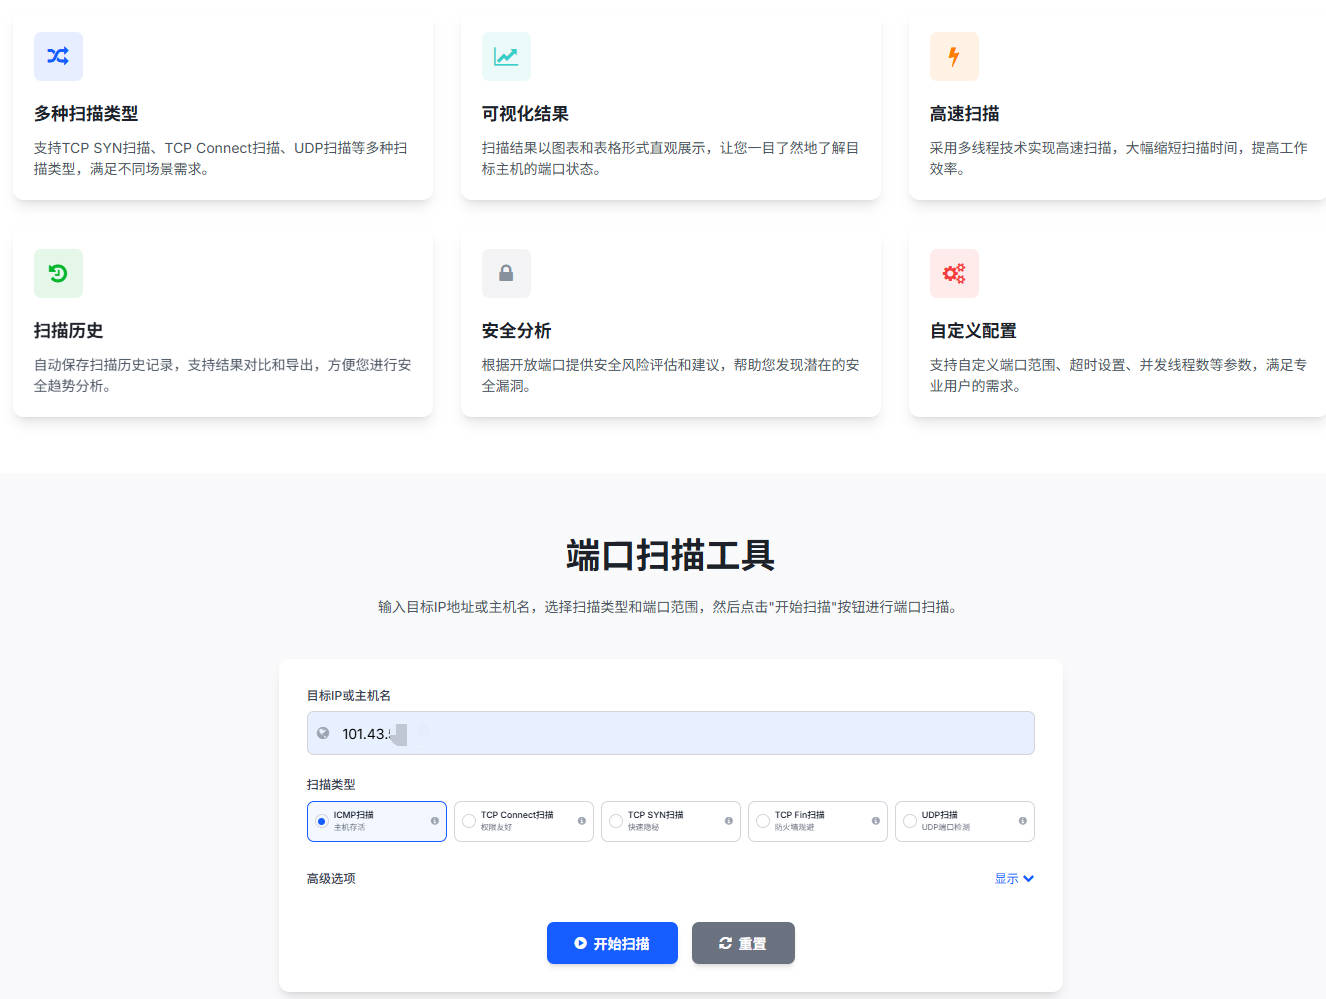
\includegraphics[width=\textwidth]{figures/icmpScan.jpg}
        \caption{ICMP测试}
        \label{fig:icmpScan}
    \end{minipage}
    \hfill
    \begin{minipage}[t]{0.48\textwidth}
        \centering
        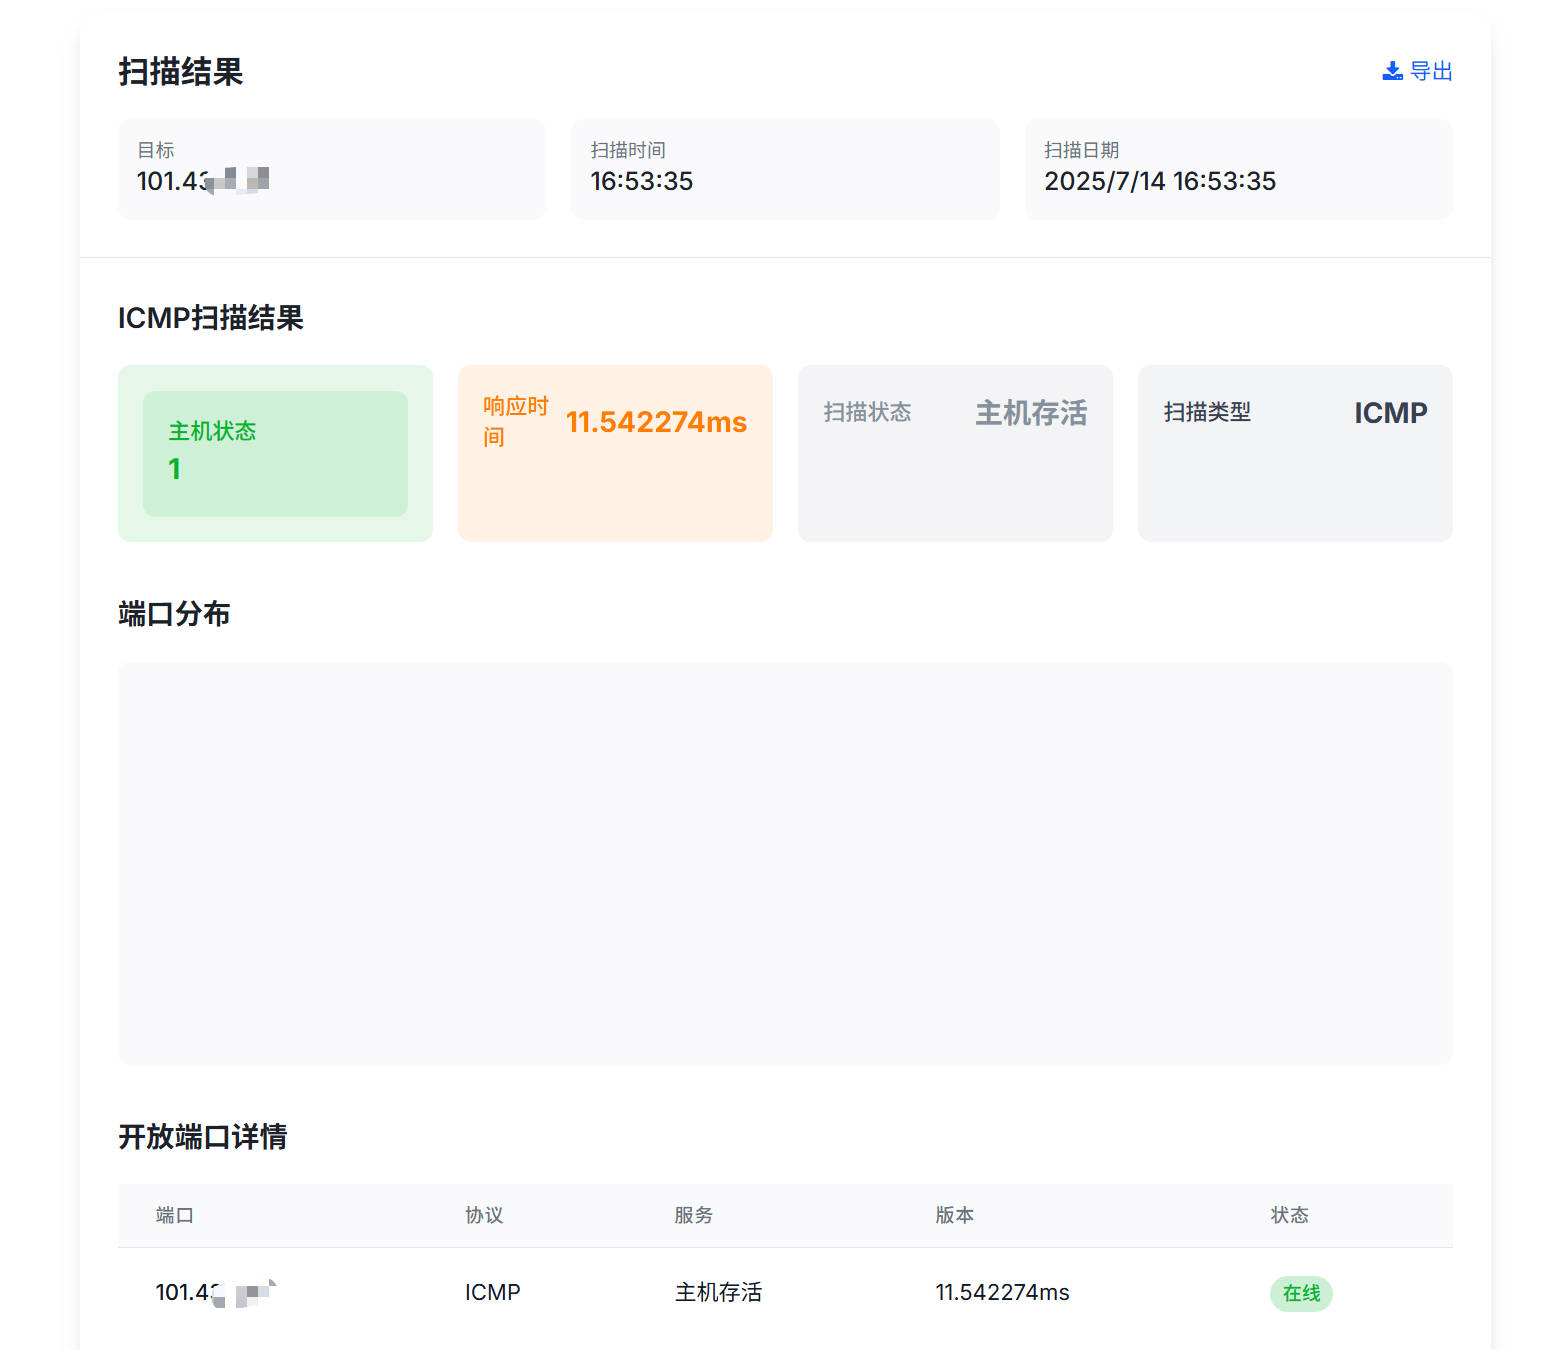
\includegraphics[width=\textwidth]{figures/icmpResult.jpg}
        \caption{ICMP结果}
        \label{fig:icmpResult}
    \end{minipage}
\end{figure}

\subsubsection{TCP Connect扫描测试}
\begin{itemize}
    \item \textbf{测试目标}:验证TCP Connect扫描对常见服务端口(如80、22、443等)的开放性检测能力。
    \item \textbf{测试环境}:本地和局域网内有Web服务、SSH服务的主机,部分端口关闭。
    \item \textbf{测试过程}:在前端输入目标IP和端口范围,选择TCP Connect扫描,观察扫描进度和结果。
    \item \textbf{测试现象}:
        \begin{itemize}
            \item 对开放的Web端口(如80、3306),扫描结果显示端口开放,能建立TCP连接。
            \item 对关闭端口,扫描结果显示端口关闭,连接被拒绝。
            \item 扫描速度受线程数影响,10线程下每秒可检测数百端口。
        \end{itemize}
    \item \textbf{测试结论}:TCP Connect扫描功能稳定,能准确区分开放与关闭端口,适合需要完整连接验证的场景。
\end{itemize}

\begin{figure}[!htbp]
    \centering
    \begin{minipage}[t]{0.48\textwidth}
        \centering
        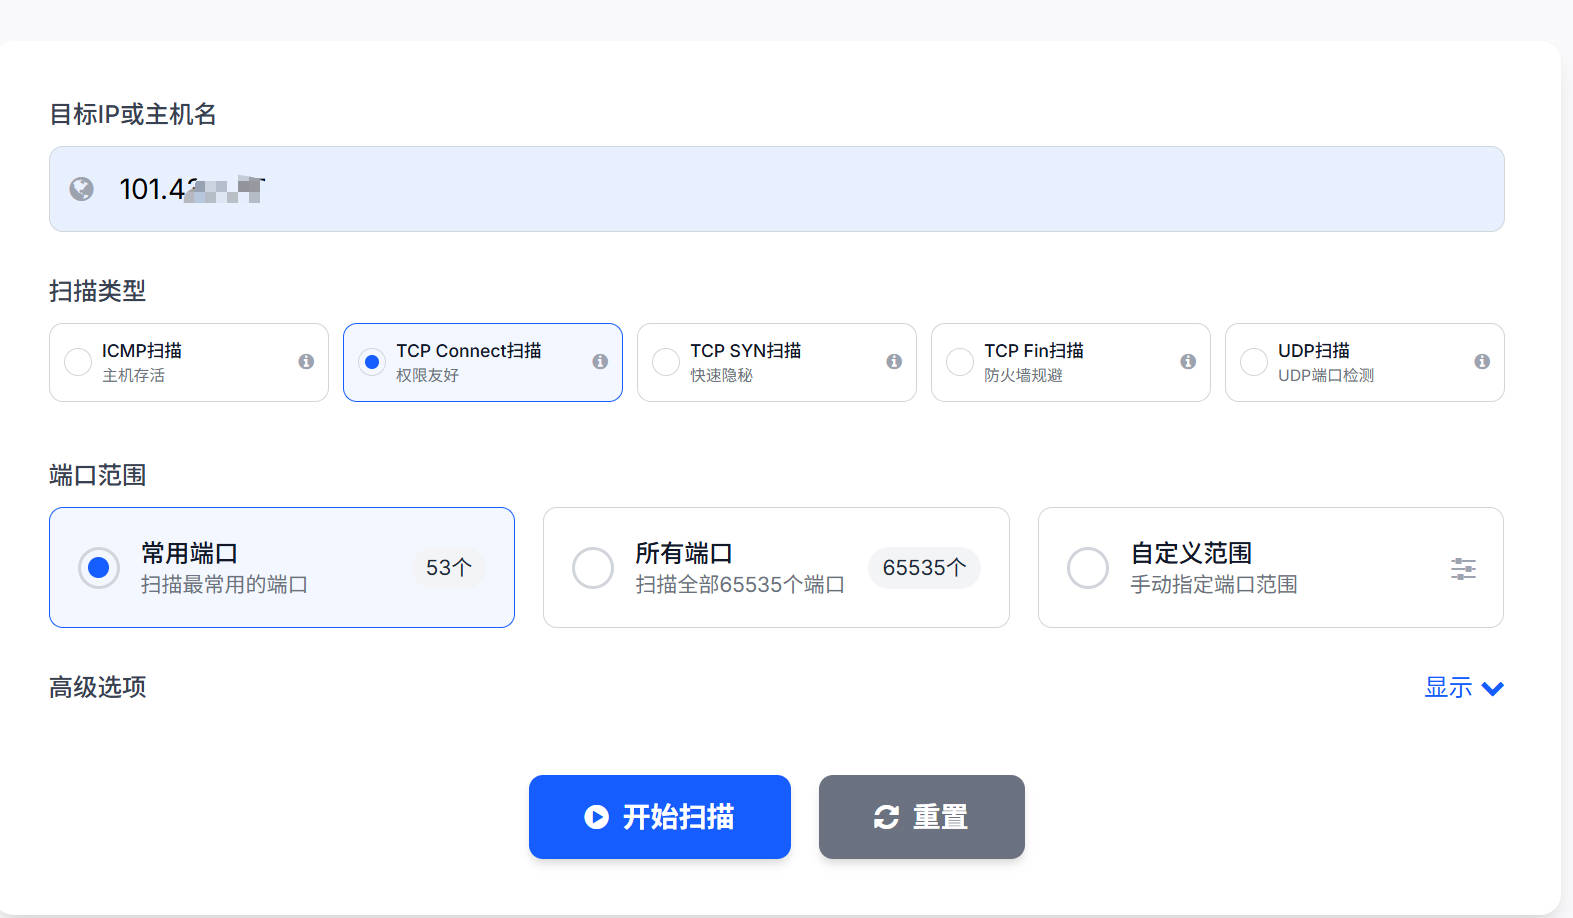
\includegraphics[width=\textwidth]{figures/connectScan.jpg}
        \caption{TCP Connect扫描}
        \label{fig:connectScan}
    \end{minipage}
    \hfill
    \begin{minipage}[t]{0.48\textwidth}
        \centering
        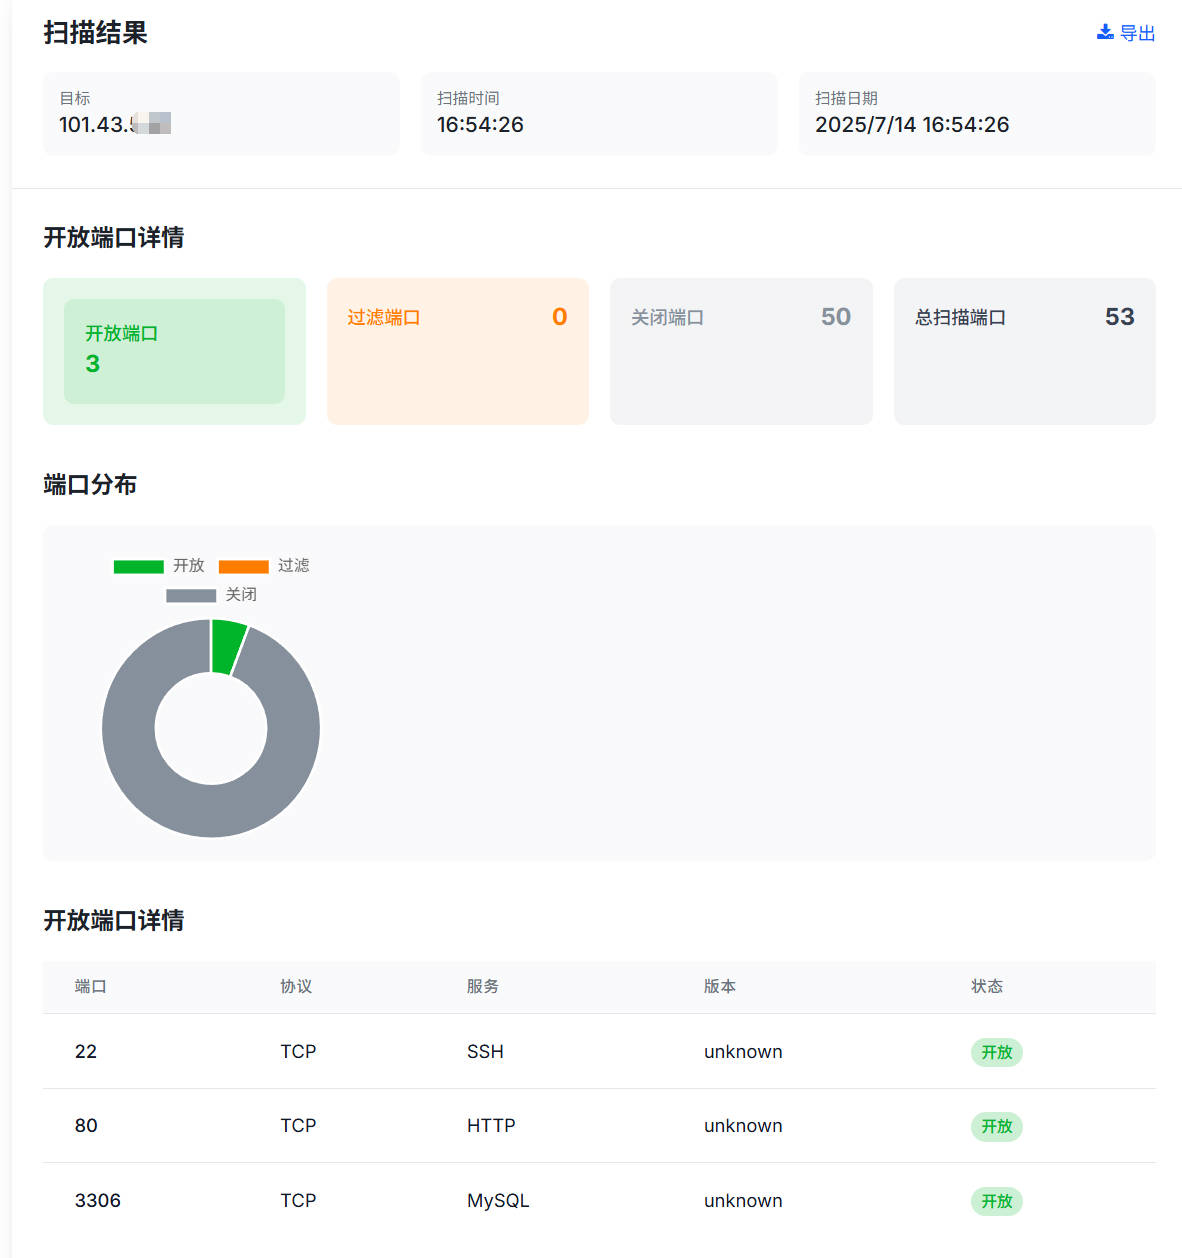
\includegraphics[width=\textwidth]{figures/connectRes.jpg}
        \caption{TCP Connect扫描结果}
        \label{fig:connectRes}
    \end{minipage}
\end{figure}

\begin{figure}[!htbp]
    \centering
    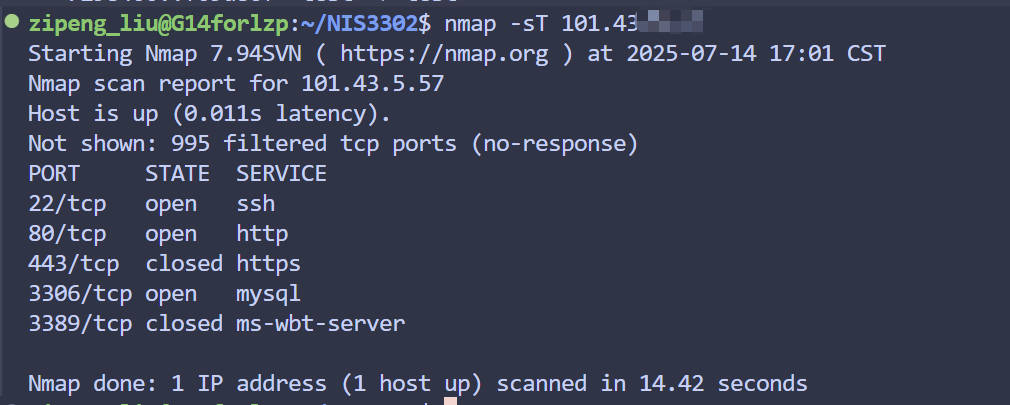
\includegraphics[width =.8\textwidth]{figures/nmap.jpg}
    \caption{nmap结果(对比)}
    \label{SJTU}
\end{figure}

\subsubsection{TCP SYN扫描测试}
\begin{itemize}
    \item \textbf{测试目标}:评估TCP SYN扫描对常用端口的快速探测能力。
    \item \textbf{测试环境}:目标主机为运行Web、SSH等服务的服务器,部分端口关闭。
    \item \textbf{测试过程}:输入目标IP和端口范围,选择SYN扫描,设置线程数为50,发起扫描。
    \item \textbf{测试现象}:
        \begin{itemize}
            \item 对开放端口,SYN扫描能快速返回开放状态,且不会建立完整连接。
            \item 对关闭端口,扫描结果准确显示端口关闭。
            \item 扫描速度快于Connect扫描,适合大范围端口探测。
        \end{itemize}
    \item \textbf{测试结论}:SYN扫描功能高效,适合大规模端口快速探测,结果与nmap等专业工具一致。
\end{itemize}

\subsubsection{TCP FIN扫描测试}
\begin{itemize}
    \item \textbf{测试目标}:测试TCP FIN扫描在不同主机和防火墙环境下的隐蔽探测能力。
    \item \textbf{测试环境}:目标主机包括普通服务器和配置有防火墙的主机。
    \item \textbf{测试过程}:输入目标IP和端口,选择FIN扫描,观察开放端口和被防火墙过滤端口的响应差异。
    \item \textbf{测试现象}:
        \begin{itemize}
            \item 对部分开放端口,FIN扫描能探测到开放状态。
            \item 某些防火墙对FIN包有特殊处理,可能导致端口状态显示为“过滤”或无响应。
            \item 与SYN扫描结果对比,部分端口表现一致,部分端口表现不同。
        \end{itemize}
    \item \textbf{测试结论}:TCP FIN扫描适合在特定网络环境下进行隐蔽探测,可辅助绕过部分防火墙检测,但对不同主机响应差异较大。
\end{itemize}

% 如有实验截图,可在下方插入:
% \begin{figure}[htbp]
%     \centering
%     \includegraphics[width=0.7\textwidth]{figures/finScan.jpg}
%     \caption{TCP FIN扫描测试结果}
%     \label{fig:finScan}
% \end{figure}

\subsubsection{UDP扫描测试}
\begin{itemize}
    \item \textbf{测试目标}:检测目标主机UDP服务端口(如DNS 53、DHCP 67/68等)的开放性。
    \item \textbf{测试环境}:目标主机为运行DNS、DHCP等UDP服务的服务器。
    \item \textbf{测试过程}:输入目标IP和UDP端口范围,选择UDP扫描,发起扫描。
    \item \textbf{测试现象}:
        \begin{itemize}
            \item 对开放的UDP端口,部分能正确识别开放状态。
            \item 对关闭端口,部分返回不可达,部分无响应(UDP协议特性)。
            \item 扫描速度受限于UDP协议和主机响应,整体慢于TCP扫描。
        \end{itemize}
    \item \textbf{测试结论}:UDP扫描可用于检测常见UDP服务端口,但受协议和网络环境影响,部分端口状态难以准确判断。
\end{itemize}


\subsubsection{Web界面测试}
\begin{itemize}
    \item \textbf{测试目标}:界面响应性、结果展示、历史记录
    \item \textbf{测试结果}:界面流畅,结果展示清晰,历史记录功能正常
    \item \textbf{测试结论}:Web界面用户体验良好,功能完整
\end{itemize}

\subsection{测试结论}
通过全面测试,系统各项功能均达到预期目标:
\begin{itemize}
    \item \textbf{功能完整性}:所有设计功能均正常实现
    \item \textbf{性能表现}:扫描速度满足实际使用需求
    \item \textbf{稳定性}:系统运行稳定,无明显bug
    \item \textbf{用户体验}:界面友好,操作简单直观
    \item \textbf{兼容性}:支持主流浏览器和操作系统
\end{itemize}

% ===================== 项目总结(详细版) =====================

\section{项目总结}

\subsection{项目成果}
本项目围绕网络安全测试需求,设计并实现了一个基于Web的多功能端口扫描工具。项目成果体现在以下几个方面:
\begin{itemize}
    \item \textbf{系统集成与功能实现}:成功集成C++高性能后端与现代Web前端,支持ICMP、TCP SYN、TCP Connect、TCP FIN、UDP等多种扫描方式,满足不同网络环境和测试需求。
    \item \textbf{高效多线程扫描}:后端实现了灵活的多线程调度机制,显著提升了大规模端口扫描的速度和效率,能够在短时间内完成对大量端口的检测。
    \item \textbf{可视化与交互体验}:前端采用响应式设计,支持实时进度显示、结果可视化(表格、图表)、历史记录管理和结果导出,极大提升了用户体验和数据分析能力。
    \item \textbf{跨平台兼容性}:系统支持主流操作系统和浏览器,便于不同用户和场景下的部署与使用。
    \item \textbf{完整测试验证}:通过功能、性能、兼容性、压力和安全等多维度测试,确保系统稳定可靠,满足实际应用需求。
\end{itemize}

\subsection{技术亮点}
\begin{itemize}
    \item \textbf{前后端分离架构}:采用RESTful API实现前后端解耦,便于系统维护、升级和扩展。
    \item \textbf{高效并发与异步处理}:后端多线程扫描与异步任务调度,有效利用多核资源,提升扫描吞吐量。
    \item \textbf{底层网络编程能力}:深入实现原始套接字、ICMP报文、TCP/UDP协议等底层网络操作,增强了系统的专业性和可控性。
    \item \textbf{数据可视化与交互}:前端集成多种可视化组件,支持动态展示扫描进度、端口分布、历史趋势等,便于用户分析和决策。
    \item \textbf{安全与健壮性设计}:接口参数校验、异常处理、权限控制等机制,保障系统安全稳定运行。
    \item \textbf{模块化与可扩展性}:各功能模块职责清晰,便于后续功能扩展和技术升级。
\end{itemize}

\subsection{项目价值}
\begin{itemize}
    \item \textbf{实用价值}:为网络安全从业者、教育工作者和普通用户提供了一个易用、高效的端口扫描和主机检测工具,适用于渗透测试、资产盘点、网络排障等多种场景。
    \item \textbf{教育与科研价值}:项目涵盖网络协议、系统编程、Web开发、并发控制等多项技术,适合作为网络安全、软件工程等课程的教学案例和实验平台。
    \item \textbf{创新与技术验证}:探索了C++与Web前端的高效集成,验证了多线程网络扫描、实时数据交互等关键技术的可行性。
    \item \textbf{团队协作与工程实践}:项目开发过程中,团队成员分工明确、协作高效,积累了宝贵的工程实践和项目管理经验。
\end{itemize}

\subsection{改进方向}
\begin{itemize}
    \item \textbf{功能扩展}:未来可增加服务版本识别、漏洞检测、分布式扫描、扫描计划定时等高级功能,进一步提升系统实用性。
    \item \textbf{性能优化}:可针对大规模目标和复杂网络环境,优化扫描算法、线程池管理和资源调度,提升极限性能。
    \item \textbf{安全增强}:引入更完善的权限认证、日志审计、防止滥用等安全机制,保障系统和用户安全。
    \item \textbf{用户体验提升}:持续优化界面设计、交互流程和移动端适配,增强系统易用性和美观性。
    \item \textbf{开放与社区建设}:可将项目开源,吸引更多开发者参与,推动功能完善和技术创新。
\end{itemize}

\section{分工}

本项目由团队成员共同完成,具体分工如下:

\begin{itemize}
    \item \textbf{项目负责人}:负责项目整体规划和进度管理
    \item \textbf{后端开发}:负责C++后端服务开发和API设计
    \item \textbf{前端开发}:负责Web界面设计和JavaScript开发
    \item \textbf{网络模块开发}:负责ICMP和端口扫描核心功能实现
    \item \textbf{测试验证}:负责系统测试和性能优化
    \item \textbf{文档编写}:负责技术文档和用户手册编写
\end{itemize}


\begin{table}[H]
\centering
\renewcommand{\arraystretch}{1.3} % 可选:增加行高
\setlength{\tabcolsep}{18pt}      % 增加列间距,默认6pt,可根据需要调整
\begin{tabular}{|p{3cm}|p{2cm}|p{5cm}|p{3cm}|}
\hline
姓名 & 是否组长 & 任务 & 评分 \\
\hline
刘梓芃 & 是 & 内容A & 说明A \\
\hline
聂鸣涛 & 否 & 内容B & 说明B \\
\hline
李卓恒 & 否 & 内容C & 说明C \\
\hline
张煜哲 & 否 & 内容D & 说明D \\
\hline
\end{tabular}
\caption{项目组成员贡献表}
\end{table}
%%----------- 参考文献 -------------------%%
%在reference.bib文件中填写参考文献,此处自动生成

% \reference


\end{document}